% Figure from MATH 591 notes, section 70. Added, not from lecture (Lecture 25): the uniform time lemma's proof on the time axis.
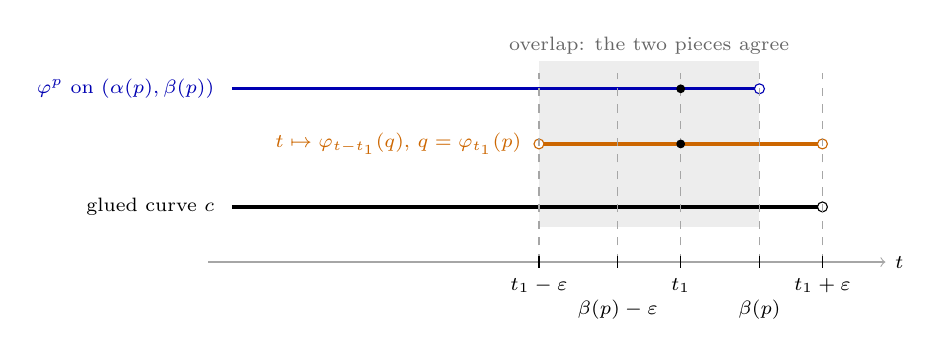
\begin{tikzpicture}[x=1cm, y=1cm]
\fill[black!7] (4.2,-0.55) rectangle (7.0,1.55);
\node[font=\scriptsize, black!60] at (5.6,1.75) {overlap: the two pieces agree};
\draw[blue!70!black, very thick] (0.3,1.2) -- (7.0,1.2); \fill[white, draw=blue!70!black] (7.0,1.2) circle (1.8pt);
\node[blue!70!black, font=\scriptsize, anchor=east] at (0.2,1.2) {$\varphi^p$ on $(\alpha(p), \beta(p))$};
\draw[orange!80!black, very thick] (4.2,0.5) -- (7.8,0.5); \fill[white, draw=orange!80!black] (4.2,0.5) circle (1.8pt); \fill[white, draw=orange!80!black] (7.8,0.5) circle (1.8pt);
\node[orange!80!black, font=\scriptsize, anchor=east] at (4.1,0.5) {$t \mapsto \varphi_{t - t_1}(q)$, $q = \varphi_{t_1}(p)$};
\draw[black, very thick] (0.3,-0.3) -- (7.8,-0.3); \fill[white, draw=black] (7.8,-0.3) circle (1.8pt);
\node[font=\scriptsize, anchor=east] at (0.2,-0.3) {glued curve $c$};
\draw[->, gray!70] (0,-1.0) -- (8.6,-1.0) node[right, font=\scriptsize, text=black] {$t$};
\foreach \x/\l in {4.2/{t_1 - \varepsilon}, 5.2/{\beta(p) - \varepsilon}, 6.0/{t_1}, 7.0/{\beta(p)}, 7.8/{t_1 + \varepsilon}} {
  \draw[black!35, dashed] (\x,-1.0) -- (\x,1.4); \draw (\x,-0.92) -- (\x,-1.08); }
\node[font=\scriptsize, below] at (4.2,-1.08) {$t_1 - \varepsilon$};
\node[font=\scriptsize, below=8pt] at (5.2,-1.08) {$\beta(p) - \varepsilon$};
\node[font=\scriptsize, below] at (6.0,-1.08) {$t_1$};
\node[font=\scriptsize, below=8pt] at (7.0,-1.08) {$\beta(p)$};
\node[font=\scriptsize, below] at (7.8,-1.08) {$t_1 + \varepsilon$};
\fill (6.0,1.2) circle (1.6pt); \fill (6.0,0.5) circle (1.6pt);
\end{tikzpicture}
